\documentclass{standalone}
\usepackage{mathpazo}
\usepackage{siunitx}
\usepackage[american voltages, american currents, american inductors]{circuitikz}
\newcommand*{\equal}{=}

\begin{document}
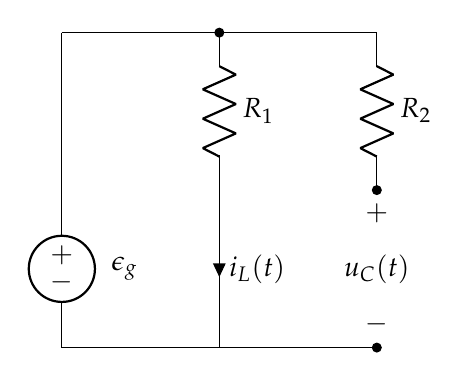
\begin{tikzpicture}
  \coordinate (A) at (0,4);
  \coordinate (B) at (2,4);
  \coordinate (C) at (4,4);
  \coordinate (D) at (0,0);
  \coordinate (E) at (2,0);
  \coordinate (F) at (4,0);
  \draw
  (A) to [short] ++(0,-2)
  to [V, v = $\epsilon_g$] (D)
  (A) to [short, -*] (B)
  to [short] (C)
  (B) to [R, l = $R_1$] ++(0, -2)
  to [short, i = $i_L(t)$] (E)
  (C) to [R, l = $R_2$] ++(0, -2)
  to [open, v^= $u_C(t)$, *-*] (F)
  (D) to [short] (F);
  \end{tikzpicture}
\end{document}